% Options for packages loaded elsewhere
\PassOptionsToPackage{unicode}{hyperref}
\PassOptionsToPackage{hyphens}{url}
%
\documentclass[
]{article}
\usepackage{amsmath,amssymb}
\usepackage{lmodern}
\usepackage{iftex}
\ifPDFTeX
  \usepackage[T1]{fontenc}
  \usepackage[utf8]{inputenc}
  \usepackage{textcomp} % provide euro and other symbols
\else % if luatex or xetex
  \usepackage{unicode-math}
  \defaultfontfeatures{Scale=MatchLowercase}
  \defaultfontfeatures[\rmfamily]{Ligatures=TeX,Scale=1}
\fi
% Use upquote if available, for straight quotes in verbatim environments
\IfFileExists{upquote.sty}{\usepackage{upquote}}{}
\IfFileExists{microtype.sty}{% use microtype if available
  \usepackage[]{microtype}
  \UseMicrotypeSet[protrusion]{basicmath} % disable protrusion for tt fonts
}{}
\makeatletter
\@ifundefined{KOMAClassName}{% if non-KOMA class
  \IfFileExists{parskip.sty}{%
    \usepackage{parskip}
  }{% else
    \setlength{\parindent}{0pt}
    \setlength{\parskip}{6pt plus 2pt minus 1pt}}
}{% if KOMA class
  \KOMAoptions{parskip=half}}
\makeatother
\usepackage{xcolor}
\usepackage[margin=1in]{geometry}
\usepackage{color}
\usepackage{fancyvrb}
\newcommand{\VerbBar}{|}
\newcommand{\VERB}{\Verb[commandchars=\\\{\}]}
\DefineVerbatimEnvironment{Highlighting}{Verbatim}{commandchars=\\\{\}}
% Add ',fontsize=\small' for more characters per line
\usepackage{framed}
\definecolor{shadecolor}{RGB}{248,248,248}
\newenvironment{Shaded}{\begin{snugshade}}{\end{snugshade}}
\newcommand{\AlertTok}[1]{\textcolor[rgb]{0.94,0.16,0.16}{#1}}
\newcommand{\AnnotationTok}[1]{\textcolor[rgb]{0.56,0.35,0.01}{\textbf{\textit{#1}}}}
\newcommand{\AttributeTok}[1]{\textcolor[rgb]{0.77,0.63,0.00}{#1}}
\newcommand{\BaseNTok}[1]{\textcolor[rgb]{0.00,0.00,0.81}{#1}}
\newcommand{\BuiltInTok}[1]{#1}
\newcommand{\CharTok}[1]{\textcolor[rgb]{0.31,0.60,0.02}{#1}}
\newcommand{\CommentTok}[1]{\textcolor[rgb]{0.56,0.35,0.01}{\textit{#1}}}
\newcommand{\CommentVarTok}[1]{\textcolor[rgb]{0.56,0.35,0.01}{\textbf{\textit{#1}}}}
\newcommand{\ConstantTok}[1]{\textcolor[rgb]{0.00,0.00,0.00}{#1}}
\newcommand{\ControlFlowTok}[1]{\textcolor[rgb]{0.13,0.29,0.53}{\textbf{#1}}}
\newcommand{\DataTypeTok}[1]{\textcolor[rgb]{0.13,0.29,0.53}{#1}}
\newcommand{\DecValTok}[1]{\textcolor[rgb]{0.00,0.00,0.81}{#1}}
\newcommand{\DocumentationTok}[1]{\textcolor[rgb]{0.56,0.35,0.01}{\textbf{\textit{#1}}}}
\newcommand{\ErrorTok}[1]{\textcolor[rgb]{0.64,0.00,0.00}{\textbf{#1}}}
\newcommand{\ExtensionTok}[1]{#1}
\newcommand{\FloatTok}[1]{\textcolor[rgb]{0.00,0.00,0.81}{#1}}
\newcommand{\FunctionTok}[1]{\textcolor[rgb]{0.00,0.00,0.00}{#1}}
\newcommand{\ImportTok}[1]{#1}
\newcommand{\InformationTok}[1]{\textcolor[rgb]{0.56,0.35,0.01}{\textbf{\textit{#1}}}}
\newcommand{\KeywordTok}[1]{\textcolor[rgb]{0.13,0.29,0.53}{\textbf{#1}}}
\newcommand{\NormalTok}[1]{#1}
\newcommand{\OperatorTok}[1]{\textcolor[rgb]{0.81,0.36,0.00}{\textbf{#1}}}
\newcommand{\OtherTok}[1]{\textcolor[rgb]{0.56,0.35,0.01}{#1}}
\newcommand{\PreprocessorTok}[1]{\textcolor[rgb]{0.56,0.35,0.01}{\textit{#1}}}
\newcommand{\RegionMarkerTok}[1]{#1}
\newcommand{\SpecialCharTok}[1]{\textcolor[rgb]{0.00,0.00,0.00}{#1}}
\newcommand{\SpecialStringTok}[1]{\textcolor[rgb]{0.31,0.60,0.02}{#1}}
\newcommand{\StringTok}[1]{\textcolor[rgb]{0.31,0.60,0.02}{#1}}
\newcommand{\VariableTok}[1]{\textcolor[rgb]{0.00,0.00,0.00}{#1}}
\newcommand{\VerbatimStringTok}[1]{\textcolor[rgb]{0.31,0.60,0.02}{#1}}
\newcommand{\WarningTok}[1]{\textcolor[rgb]{0.56,0.35,0.01}{\textbf{\textit{#1}}}}
\usepackage{graphicx}
\makeatletter
\def\maxwidth{\ifdim\Gin@nat@width>\linewidth\linewidth\else\Gin@nat@width\fi}
\def\maxheight{\ifdim\Gin@nat@height>\textheight\textheight\else\Gin@nat@height\fi}
\makeatother
% Scale images if necessary, so that they will not overflow the page
% margins by default, and it is still possible to overwrite the defaults
% using explicit options in \includegraphics[width, height, ...]{}
\setkeys{Gin}{width=\maxwidth,height=\maxheight,keepaspectratio}
% Set default figure placement to htbp
\makeatletter
\def\fps@figure{htbp}
\makeatother
\setlength{\emergencystretch}{3em} % prevent overfull lines
\providecommand{\tightlist}{%
  \setlength{\itemsep}{0pt}\setlength{\parskip}{0pt}}
\setcounter{secnumdepth}{-\maxdimen} % remove section numbering
\ifLuaTeX
  \usepackage{selnolig}  % disable illegal ligatures
\fi
\IfFileExists{bookmark.sty}{\usepackage{bookmark}}{\usepackage{hyperref}}
\IfFileExists{xurl.sty}{\usepackage{xurl}}{} % add URL line breaks if available
\urlstyle{same} % disable monospaced font for URLs
\hypersetup{
  pdftitle={tp2},
  pdfauthor={Lapu Matthias \textbar{} Amaël Kreis},
  hidelinks,
  pdfcreator={LaTeX via pandoc}}

\title{tp2}
\author{Lapu Matthias \textbar{} Amaël Kreis}
\date{2023-02-17}

\begin{document}
\maketitle

\hypertarget{i.-variation-sous-jacente-et-uxe9chantillonnage-ruxe9puxe9tuxe9}{%
\subsection{I. Variation sous-jacente et échantillonnage
répété}\label{i.-variation-sous-jacente-et-uxe9chantillonnage-ruxe9puxe9tuxe9}}

\begin{enumerate}
\def\labelenumi{\arabic{enumi}.}
\tightlist
\item
  Si X ∼ E(0.5), quelle est la probabilité qu'on observe une valeur
  supérieure à 3?
\end{enumerate}

2.Simulez un échantillon de taille n = 20 d'un loi de E(0,5), créez un
histogramme de votre échantillon et commentez la forme de votre
histogramme. Superposer la vrai densité. Quelle est la probabilité
empirique qu'on observe une valeur supérieure à 3 ?

\begin{Shaded}
\begin{Highlighting}[]
\NormalTok{x}\OtherTok{\textless{}{-}}\FunctionTok{rexp}\NormalTok{(}\DecValTok{20}\NormalTok{,}\FloatTok{0.5}\NormalTok{)}
\FunctionTok{hist}\NormalTok{(x, }\AttributeTok{freq=}\ConstantTok{FALSE}\NormalTok{)}
\NormalTok{maxvalue }\OtherTok{\textless{}{-}} \FunctionTok{ceiling}\NormalTok{(}\FunctionTok{max}\NormalTok{(x))}
\FunctionTok{lines}\NormalTok{(}\DecValTok{0}\SpecialCharTok{:}\NormalTok{maxvalue,}\FunctionTok{dexp}\NormalTok{(}\DecValTok{0}\SpecialCharTok{:}\NormalTok{maxvalue, }\FloatTok{0.5}\NormalTok{), }\AttributeTok{col=}\StringTok{"green"}\NormalTok{,)}
\end{Highlighting}
\end{Shaded}

\includegraphics{tp2_files/figure-latex/unnamed-chunk-1-1.pdf}

Commentaire histogramme à insérer

3.Répétez cette opération 5 ou 6 fois et commentez les différences entre
les histogrammes que vous obtenez à chaque fois. Utilisez la même limite
sur les axes pour faciliter la comparaison. Notez également comment la
probabilité empirique qu'on observe une valeur supérieure à 3 change.

\begin{enumerate}
\def\labelenumi{\arabic{enumi}.}
\setcounter{enumi}{3}
\tightlist
\item
  Augmentez la taille de votre échantillon à 100 et répétez votre
  expérience. Que remarquez-vous?
\end{enumerate}

\includegraphics{tp2_files/figure-latex/unnamed-chunk-3-1.pdf}

\hypertarget{ii.-variabilituxe9-aluxe9atoire-du-maximum-de-luxe9chantillon}{%
\subsection{II. Variabilité aléatoire du maximum de
l'échantillon}\label{ii.-variabilituxe9-aluxe9atoire-du-maximum-de-luxe9chantillon}}

\hypertarget{simuler-un-uxe9chantillon-de-taille-n-10-dune-loi-u1-1-et-enregistrez-le-maximum-de-luxe9chantillon.}{%
\section{1. Simuler un échantillon de taille n = 10 d'une loi U(−1, 1)
et enregistrez le maximum de
l'échantillon.}\label{simuler-un-uxe9chantillon-de-taille-n-10-dune-loi-u1-1-et-enregistrez-le-maximum-de-luxe9chantillon.}}

\begin{Shaded}
\begin{Highlighting}[]
\NormalTok{x }\OtherTok{\textless{}{-}} \FunctionTok{runif}\NormalTok{(}\DecValTok{10}\NormalTok{, }\SpecialCharTok{{-}}\DecValTok{1}\NormalTok{, }\DecValTok{1}\NormalTok{)}
\NormalTok{max }\OtherTok{\textless{}{-}} \FunctionTok{max}\NormalTok{(x)}
\end{Highlighting}
\end{Shaded}

\hypertarget{ruxe9puxe9tez-les-deux-uxe9tapes-ci-dessus-dix-fois-en-uxe9crivant-le-maximum-de-luxe9chantillon-uxe0-chaque-fois.-commentez-la-variabilituxe9-des-valeurs-que-vous-obtenez-pour-les-maxima-de-votre-uxe9chantillon.}{%
\section{2. Répétez les deux étapes ci-dessus dix fois, en écrivant le
maximum de l'échantillon à chaque fois. Commentez la variabilité des
valeurs que vous obtenez pour les maxima de votre
échantillon.}\label{ruxe9puxe9tez-les-deux-uxe9tapes-ci-dessus-dix-fois-en-uxe9crivant-le-maximum-de-luxe9chantillon-uxe0-chaque-fois.-commentez-la-variabilituxe9-des-valeurs-que-vous-obtenez-pour-les-maxima-de-votre-uxe9chantillon.}}

\begin{Shaded}
\begin{Highlighting}[]
\ControlFlowTok{for}\NormalTok{ (i }\ControlFlowTok{in} \DecValTok{1}\SpecialCharTok{:}\DecValTok{10}\NormalTok{) \{}
\NormalTok{  x }\OtherTok{\textless{}{-}} \FunctionTok{runif}\NormalTok{(}\DecValTok{10}\NormalTok{, }\SpecialCharTok{{-}}\DecValTok{1}\NormalTok{, }\DecValTok{1}\NormalTok{)}
\NormalTok{\}}
\end{Highlighting}
\end{Shaded}

\hypertarget{ruxe9puxe9tez-100-fois-et-construisez-un-histogramme-et-une-bouxeete-uxe0-moustaches.-quelle-est-la-loi-dumaximum-m-max-1in-x-i-ouxf9-x-i-u1-1-td1-superposer-la-densituxe9-thuxe9oreique-sur-lhistogramme.-que-remarquez-vous}{%
\section{3. Répétez 100 fois et construisez un histogramme et une boîte
à moustaches. Quelle est la loi dumaximum, M = max 1≤i≤n X i où X i ∼
U(−1, 1) (TD1) ? Superposer la densité théoreique sur l'histogramme. Que
remarquez-vous
?}\label{ruxe9puxe9tez-100-fois-et-construisez-un-histogramme-et-une-bouxeete-uxe0-moustaches.-quelle-est-la-loi-dumaximum-m-max-1in-x-i-ouxf9-x-i-u1-1-td1-superposer-la-densituxe9-thuxe9oreique-sur-lhistogramme.-que-remarquez-vous}}

\begin{Shaded}
\begin{Highlighting}[]
\FunctionTok{par}\NormalTok{(}\AttributeTok{mfrow=}\FunctionTok{c}\NormalTok{(}\DecValTok{3}\NormalTok{,}\DecValTok{4}\NormalTok{))}
\ControlFlowTok{for}\NormalTok{ (i }\ControlFlowTok{in} \DecValTok{1}\SpecialCharTok{:}\DecValTok{100}\NormalTok{) \{}
\NormalTok{  x }\OtherTok{\textless{}{-}} \FunctionTok{runif}\NormalTok{(}\DecValTok{10}\NormalTok{, }\SpecialCharTok{{-}}\DecValTok{1}\NormalTok{, }\DecValTok{1}\NormalTok{)}
  \FunctionTok{hist}\NormalTok{(x)}
  \FunctionTok{boxplot}\NormalTok{(x, }\AttributeTok{horizontal =} \ConstantTok{TRUE}\NormalTok{)}
\NormalTok{\}}
\end{Highlighting}
\end{Shaded}

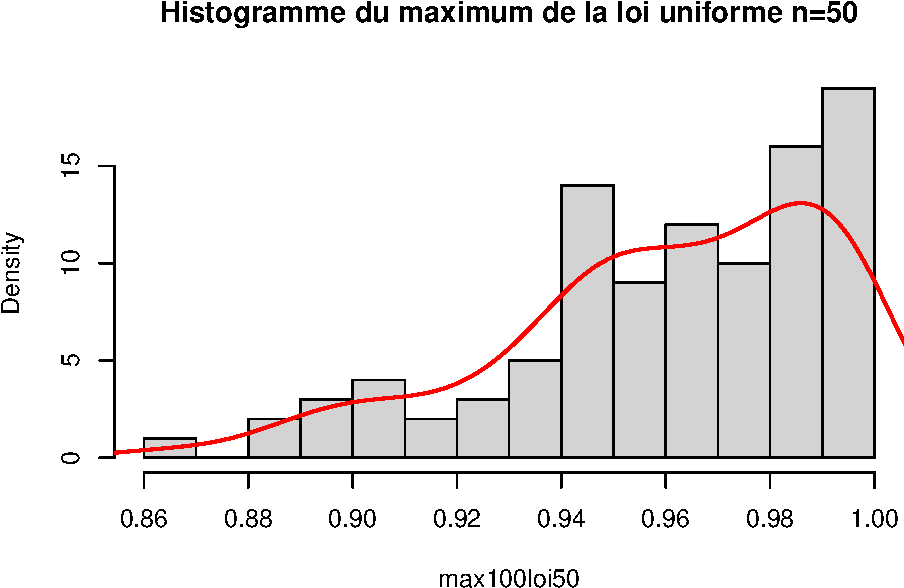
\includegraphics{tp2_files/figure-latex/unnamed-chunk-6-1.pdf}
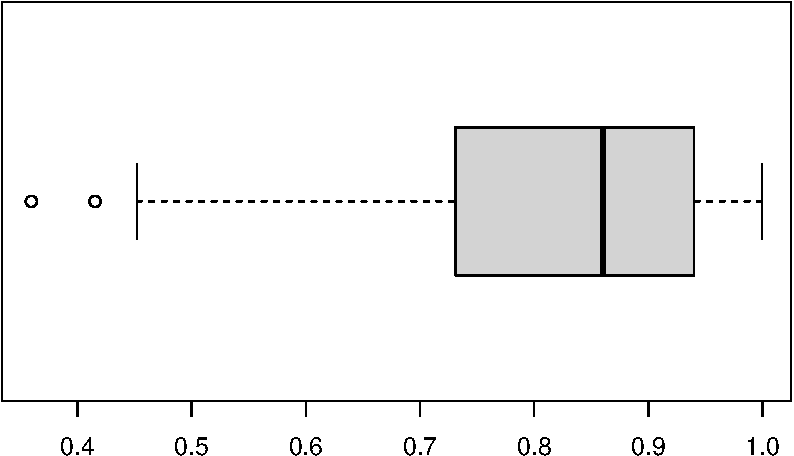
\includegraphics{tp2_files/figure-latex/unnamed-chunk-6-2.pdf}
\includegraphics{tp2_files/figure-latex/unnamed-chunk-6-3.pdf}
\includegraphics{tp2_files/figure-latex/unnamed-chunk-6-4.pdf}
\includegraphics{tp2_files/figure-latex/unnamed-chunk-6-5.pdf}
\includegraphics{tp2_files/figure-latex/unnamed-chunk-6-6.pdf}
\includegraphics{tp2_files/figure-latex/unnamed-chunk-6-7.pdf}
\includegraphics{tp2_files/figure-latex/unnamed-chunk-6-8.pdf}
\includegraphics{tp2_files/figure-latex/unnamed-chunk-6-9.pdf}
\includegraphics{tp2_files/figure-latex/unnamed-chunk-6-10.pdf}
\includegraphics{tp2_files/figure-latex/unnamed-chunk-6-11.pdf}
\includegraphics{tp2_files/figure-latex/unnamed-chunk-6-12.pdf}
\includegraphics{tp2_files/figure-latex/unnamed-chunk-6-13.pdf}
\includegraphics{tp2_files/figure-latex/unnamed-chunk-6-14.pdf}
\includegraphics{tp2_files/figure-latex/unnamed-chunk-6-15.pdf}
\includegraphics{tp2_files/figure-latex/unnamed-chunk-6-16.pdf}
\includegraphics{tp2_files/figure-latex/unnamed-chunk-6-17.pdf}

\hypertarget{augmentez-la-taille-de-votre-uxe9chantillon-uxe0-50-et-ruxe9puxe9tez-votre-expuxe9rience.-que-remarquez-vous-sont-ils-proches-de-la-symuxe9trie}{%
\section{4. Augmentez la taille de votre échantillon à 50 et répétez
votre expérience. Que remarquez-vous? Sont-ils proches de la symétrie
?}\label{augmentez-la-taille-de-votre-uxe9chantillon-uxe0-50-et-ruxe9puxe9tez-votre-expuxe9rience.-que-remarquez-vous-sont-ils-proches-de-la-symuxe9trie}}

\begin{Shaded}
\begin{Highlighting}[]
\NormalTok{x }\OtherTok{\textless{}{-}} \FunctionTok{runif}\NormalTok{(}\DecValTok{50}\NormalTok{, }\SpecialCharTok{{-}}\DecValTok{1}\NormalTok{, }\DecValTok{1}\NormalTok{)}
\end{Highlighting}
\end{Shaded}

\hypertarget{monte-carlo-methods}{%
\subsection{Monte Carlo Methods}\label{monte-carlo-methods}}

\hypertarget{moyenne-et-phuxe9nomuxe8ne-de-concentration.}{%
\section{Moyenne et phénomène de
concentration.}\label{moyenne-et-phuxe9nomuxe8ne-de-concentration.}}

\begin{enumerate}
\def\labelenumi{\arabic{enumi}.}
\tightlist
\item
  Supposons que la variance σ2 = V {[}ψ(X){]} \textless{} ∞. Donner une
  borne de cette quantité en utilisant l'inégalité de Bienaymé
  Chebychev.
\end{enumerate}

On trouve grace à l'inégalité de Bienaymé Chebychev:

\[
a^{2}P(|\psi(X) - \theta| \ge a) \le V[\psi(X)]
\]

2. En supposant que a ≤ ψ(Xi) ≤ b, donner une borne en utilisant
l'inégalité de Hoeffding.

\[
On\;a:\;S_{n} = \sum_{k=1}^{n}\psi(X)=n\psi(X)
\]

\[
P(|S_{n}-E(S_{n})| \ge t) \le 2exp(-\frac{2t^{2}}{\sum_{k=1}^{n}(b-a)^{2}})
\]

\[
\Leftrightarrow 
P(|n\psi(X)-n\theta| \ge t) \le 2exp(-\frac{2t^{2}}{n(b-a)^{2}})
\]

\[
\Leftrightarrow 
P(|\psi(X)-\theta| \ge u) \le 2exp(-\frac{2nu^{2}}{(b-a)^{2}})
\]

\hypertarget{thuxe9oruxe8me-central-limite-et-estimation-monte-carlo}{%
\subsection{Théorème Central Limite et Estimation Monte
Carlo}\label{thuxe9oruxe8me-central-limite-et-estimation-monte-carlo}}

1. Vérifier que l'espérance théorique d'une loi de Pareto est E {[}X{]}
= αa/α−1.

\[
P(X\le t)= (1-\left( \frac{a}{t} \right)^{\alpha}) , \;avec \;x \ge a
\]

Donc

\[
E(X) = \int_{0}^{+\infty}1-P(X\le t)dt = \int_{0}^{+\infty}P(X\gt t)dt
\]

\[
=a+a^{\alpha}\int_{a}^{+\infty}\frac{1}{t^{\alpha}}dt=a + \frac{a}{\alpha -1} =\frac{\alpha a}{\alpha -1}
\]

2. Simuler N = 1000 échantillons i.i.d de loi commune Pareto P(a, α)
(avec votre choix de paramètres)

de taille n = 5, 30, 100 et calculer les moyennes et variances
empiriques ¯Xn,i et Sn,i, i = 1, . . . ,N.

\begin{verbatim}
## 
## Attachement du package : 'EnvStats'
\end{verbatim}

\begin{verbatim}
## Les objets suivants sont masqués depuis 'package:stats':
## 
##     predict, predict.lm
\end{verbatim}

\begin{verbatim}
## L'objet suivant est masqué depuis 'package:base':
## 
##     print.default
\end{verbatim}

\begin{verbatim}
## [1] "Moyenne empirique n = 5"
\end{verbatim}

\begin{verbatim}
## [1] 1.479070 1.513297 1.461963 1.491601 1.472541
\end{verbatim}

\begin{verbatim}
## [1] "Moyenne empirique n = 30"
\end{verbatim}

\begin{verbatim}
##  [1] 1.492730 1.490853 1.518382 1.459188 1.484109 1.490997 1.515904 1.493364
##  [9] 1.459353 1.485976 1.519345 1.454689 1.508880 1.475957 1.498536 1.460600
## [17] 1.480212 1.470221 1.480086 1.506799 1.498481 1.579768 1.533892 1.527462
## [25] 1.569267 1.501870 1.522958 1.485226 1.529034 1.538133
\end{verbatim}

\begin{verbatim}
## [1] "Moyenne empirique n = 100"
\end{verbatim}

\begin{verbatim}
##   [1] 1.481298 1.544367 1.474200 1.536694 1.567344 1.508928 1.558064 1.486939
##   [9] 1.496005 1.467260 1.490799 1.515588 1.493461 1.513691 1.485057 1.510824
##  [17] 1.477423 1.498575 1.517541 1.537846 1.445613 1.531868 1.504366 1.485822
##  [25] 1.514643 1.490130 1.505432 1.480597 1.502357 1.485207 1.501143 1.535528
##  [33] 1.523921 1.543857 1.542164 1.456337 1.484615 1.500274 1.482810 1.526243
##  [41] 1.484604 1.530666 1.524066 1.479331 1.483951 1.495713 1.458394 1.516140
##  [49] 1.476872 1.531987 1.519867 1.504368 1.492814 1.482882 1.507432 1.483867
##  [57] 1.502059 1.468874 1.467594 1.494807 1.518294 1.472056 1.564442 1.481049
##  [65] 1.490093 1.524345 1.489757 1.535153 1.487791 1.564464 1.480847 1.465269
##  [73] 1.511971 1.505830 1.481756 1.482172 1.472652 1.477693 1.529220 1.524099
##  [81] 1.491203 1.512400 1.537463 1.516096 1.521223 1.495108 1.512389 1.502470
##  [89] 1.514787 1.519197 1.517017 1.582732 1.478491 1.504561 1.491144 1.516476
##  [97] 1.519475 1.546534 1.482847 1.495771
\end{verbatim}

\begin{verbatim}
## [1] "Variance empirique n = 5"
\end{verbatim}

\begin{verbatim}
## [1] 0.002187649 0.002290068 0.002137337 0.002224873 0.002168376
\end{verbatim}

\begin{verbatim}
## [1] "Variance empirique n = 30"
\end{verbatim}

\begin{verbatim}
##  [1] 0.002228243 0.002222642 0.002305484 0.002129228 0.002202580 0.002223071
##  [7] 0.002297965 0.002230137 0.002129711 0.002208123 0.002308409 0.002116119
## [13] 0.002276720 0.002178449 0.002245610 0.002133352 0.002191026 0.002161550
## [19] 0.002190654 0.002270442 0.002245446 0.002495668 0.002352824 0.002333142
## [25] 0.002462600 0.002255614 0.002319400 0.002205895 0.002337946 0.002365854
\end{verbatim}

\begin{verbatim}
## [1] "Variance empirique n = 100"
\end{verbatim}

\begin{verbatim}
##   [1] 0.002194243 0.002385071 0.002173265 0.002361429 0.002456568 0.002276864
##   [7] 0.002427564 0.002210987 0.002238030 0.002152851 0.002222481 0.002297006
##  [13] 0.002230425 0.002291259 0.002205394 0.002282590 0.002182778 0.002245726
##  [19] 0.002302929 0.002364969 0.002089797 0.002346618 0.002263117 0.002207668
##  [25] 0.002294145 0.002220488 0.002266326 0.002192167 0.002257075 0.002205841
##  [31] 0.002253431 0.002357845 0.002322336 0.002383496 0.002378271 0.002120917
##  [37] 0.002204081 0.002250821 0.002198725 0.002329418 0.002204049 0.002342938
##  [43] 0.002322778 0.002188419 0.002202111 0.002237157 0.002126913 0.002298682
##  [49] 0.002181151 0.002346985 0.002309997 0.002263122 0.002228495 0.002198939
##  [55] 0.002272351 0.002201862 0.002256181 0.002157590 0.002153833 0.002234447
##  [61] 0.002305217 0.002166947 0.002447480 0.002193505 0.002220376 0.002323627
##  [67] 0.002219376 0.002356694 0.002213523 0.002447548 0.002192908 0.002147014
##  [73] 0.002286057 0.002267525 0.002195601 0.002196834 0.002168705 0.002183577
##  [79] 0.002338514 0.002322878 0.002223686 0.002287353 0.002363794 0.002298547
##  [85] 0.002314120 0.002235347 0.002287322 0.002257417 0.002294581 0.002307958
##  [91] 0.002301339 0.002505041 0.002185937 0.002263702 0.002223510 0.002299700
##  [97] 0.002308805 0.002391769 0.002198834 0.002237330
\end{verbatim}

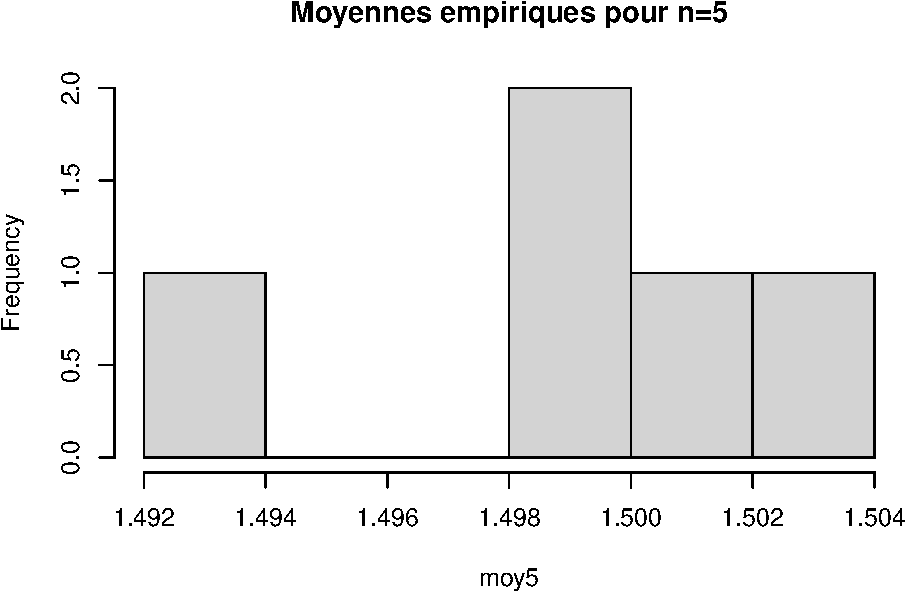
\includegraphics{tp2_files/figure-latex/echantillons-1.pdf}
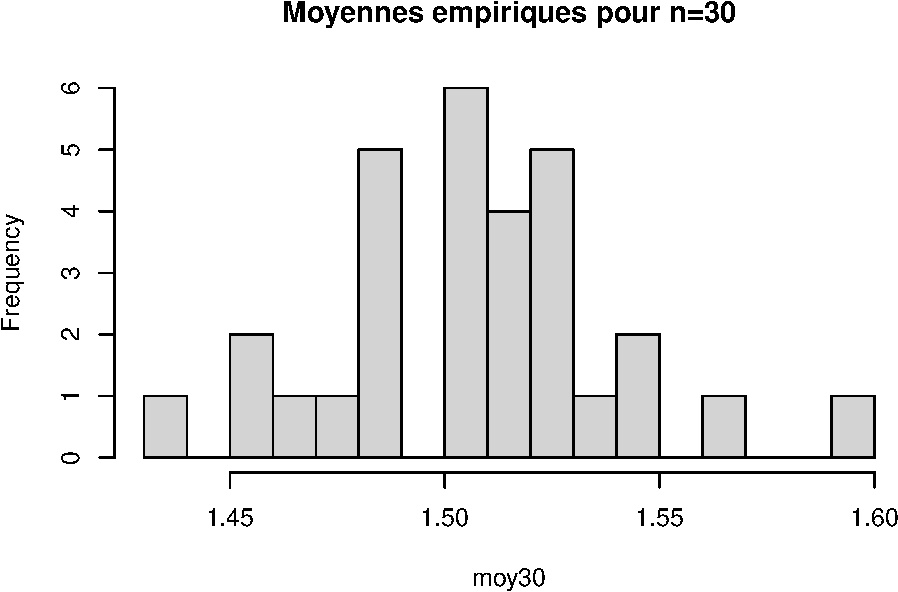
\includegraphics{tp2_files/figure-latex/echantillons-2.pdf}
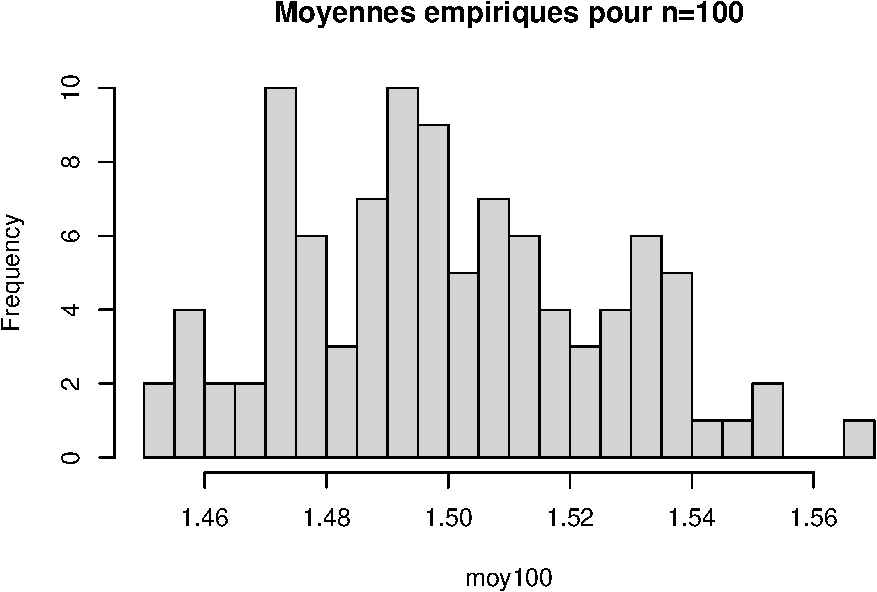
\includegraphics{tp2_files/figure-latex/echantillons-3.pdf}

\begin{enumerate}
\def\labelenumi{\arabic{enumi}.}
\setcounter{enumi}{3}
\tightlist
\item
  A l'aide d'une renormalisation adéquate (an, bn), montrer que Un,i =
  ¯Xn,i−an/ bn a une loi que vous pouvez approchez. Comparez histogramme
  de les moyennes empiriques normalisées, Un,i, et distribution
  théorique approchée. Quelle est l'influence de la taille de
  l'échantillon n sur la qualité de cette approximation?
\end{enumerate}

\begin{Shaded}
\begin{Highlighting}[]
\NormalTok{moy5CentreeReduite }\OtherTok{\textless{}{-}}\NormalTok{ (moy5}\SpecialCharTok{{-}}\FunctionTok{mean}\NormalTok{(moy5))}\SpecialCharTok{/}\FunctionTok{mean}\NormalTok{(moy5}\SpecialCharTok{\^{}}\DecValTok{2}\SpecialCharTok{/}\DecValTok{1000}\NormalTok{)}
\NormalTok{moy30CentreeReduite }\OtherTok{\textless{}{-}}\NormalTok{ (moy30}\SpecialCharTok{{-}}\FunctionTok{mean}\NormalTok{(moy30))}\SpecialCharTok{/}\FunctionTok{mean}\NormalTok{(moy30}\SpecialCharTok{\^{}}\DecValTok{2}\SpecialCharTok{/}\DecValTok{1000}\NormalTok{)}
\NormalTok{moy100CentreeReduite }\OtherTok{\textless{}{-}}\NormalTok{ (moy100}\SpecialCharTok{{-}}\FunctionTok{mean}\NormalTok{(moy100))}\SpecialCharTok{/}\FunctionTok{mean}\NormalTok{(moy100}\SpecialCharTok{\^{}}\DecValTok{2}\SpecialCharTok{/}\DecValTok{1000}\NormalTok{)}

\FunctionTok{hist}\NormalTok{(moy5CentreeReduite,}\AttributeTok{breaks =} \DecValTok{5}\NormalTok{)}
\end{Highlighting}
\end{Shaded}

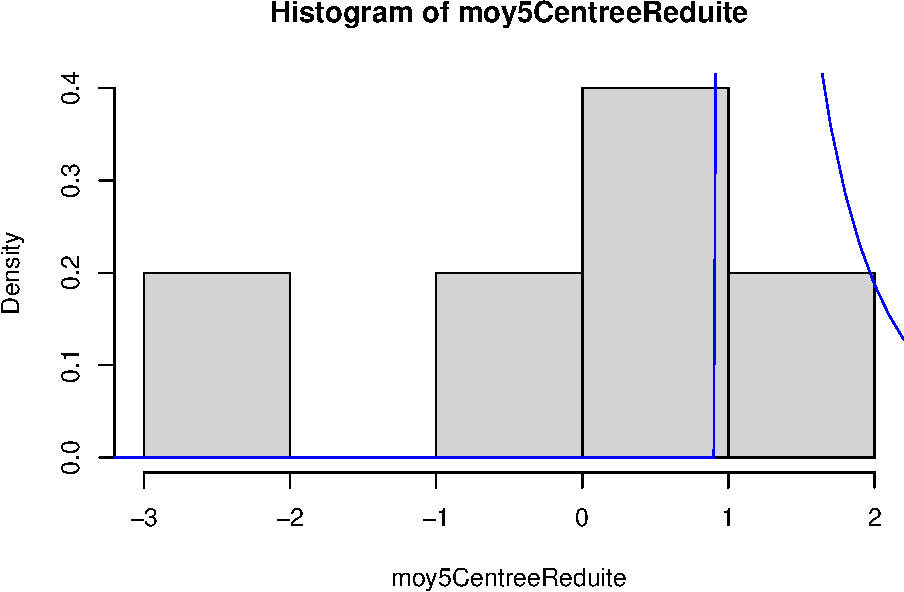
\includegraphics{tp2_files/figure-latex/normalisation-1.pdf}

\begin{Shaded}
\begin{Highlighting}[]
\FunctionTok{hist}\NormalTok{(moy30CentreeReduite,}\AttributeTok{breaks =} \DecValTok{30}\NormalTok{)}
\end{Highlighting}
\end{Shaded}

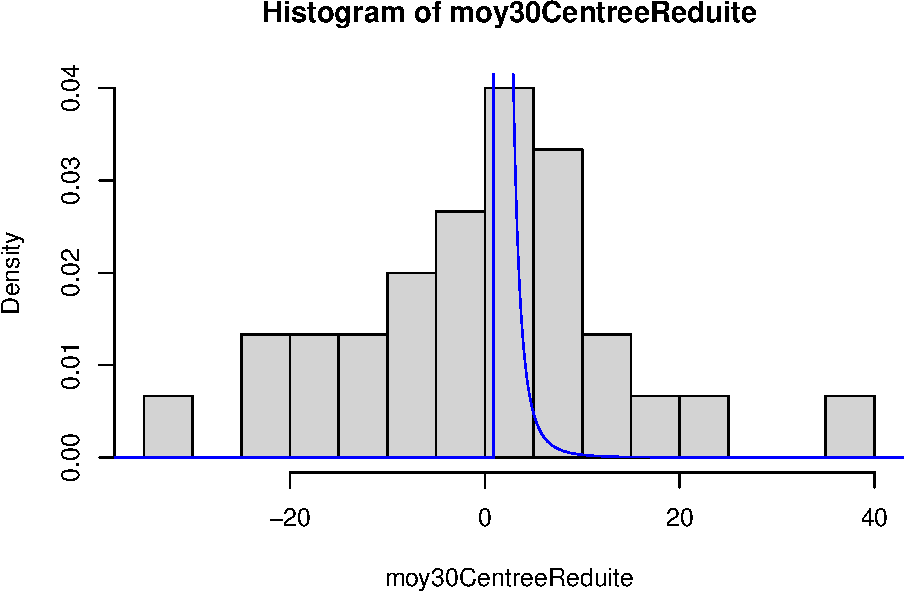
\includegraphics{tp2_files/figure-latex/normalisation-2.pdf}

\begin{Shaded}
\begin{Highlighting}[]
\FunctionTok{hist}\NormalTok{(moy100CentreeReduite,}\AttributeTok{breaks =} \DecValTok{100}\NormalTok{)}
\end{Highlighting}
\end{Shaded}

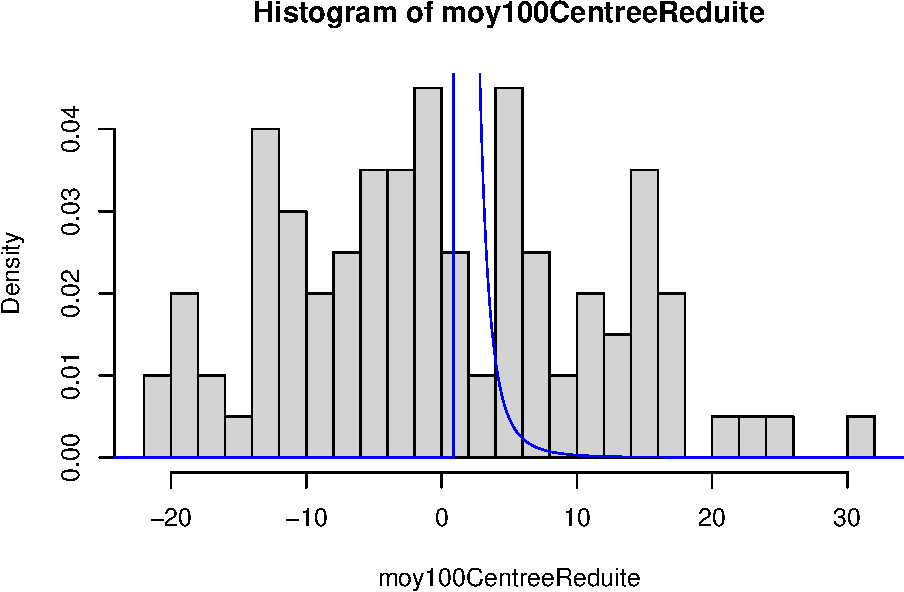
\includegraphics{tp2_files/figure-latex/normalisation-3.pdf}

\hypertarget{quand-le-thuxe9oruxe8me-de-central-limite-ne-sapplique-pas}{%
\subsection{Quand le théorème de central limite ne s'applique
pas}\label{quand-le-thuxe9oruxe8me-de-central-limite-ne-sapplique-pas}}

1. Simuler un échantillon de taille n = 20 d'une loi de C(2) et calculer
la moyenne empirique ¯Xn.

Moyenne empirique:

\begin{Shaded}
\begin{Highlighting}[]
\FunctionTok{print}\NormalTok{(}\FunctionTok{mean}\NormalTok{(}\FunctionTok{rcauchy}\NormalTok{(}\DecValTok{20}\NormalTok{,}\DecValTok{2}\NormalTok{,}\DecValTok{1}\NormalTok{)))}
\end{Highlighting}
\end{Shaded}

\begin{verbatim}
## [1] 1.400194
\end{verbatim}

2. Faites varier la taille de l'échantillon n = 20, 100, 1000 et 10000.
Qu'en déduire ?

\begin{Shaded}
\begin{Highlighting}[]
\FunctionTok{print}\NormalTok{(}\FunctionTok{mean}\NormalTok{(}\FunctionTok{rcauchy}\NormalTok{(}\DecValTok{20}\NormalTok{,}\DecValTok{2}\NormalTok{,}\DecValTok{1}\NormalTok{)))}
\end{Highlighting}
\end{Shaded}

\begin{verbatim}
## [1] 2.203773
\end{verbatim}

\begin{Shaded}
\begin{Highlighting}[]
\FunctionTok{print}\NormalTok{(}\FunctionTok{mean}\NormalTok{(}\FunctionTok{rcauchy}\NormalTok{(}\DecValTok{100}\NormalTok{,}\DecValTok{2}\NormalTok{,}\DecValTok{1}\NormalTok{)))}
\end{Highlighting}
\end{Shaded}

\begin{verbatim}
## [1] 2.411406
\end{verbatim}

\begin{Shaded}
\begin{Highlighting}[]
\FunctionTok{print}\NormalTok{(}\FunctionTok{mean}\NormalTok{(}\FunctionTok{rcauchy}\NormalTok{(}\DecValTok{1000}\NormalTok{,}\DecValTok{2}\NormalTok{,}\DecValTok{1}\NormalTok{)))}
\end{Highlighting}
\end{Shaded}

\begin{verbatim}
## [1] 1.047212
\end{verbatim}

\begin{Shaded}
\begin{Highlighting}[]
\FunctionTok{print}\NormalTok{(}\FunctionTok{mean}\NormalTok{(}\FunctionTok{rcauchy}\NormalTok{(}\DecValTok{10000}\NormalTok{,}\DecValTok{2}\NormalTok{,}\DecValTok{1}\NormalTok{)))}
\end{Highlighting}
\end{Shaded}

\begin{verbatim}
## [1] 2.090977
\end{verbatim}

\end{document}
